% Dokumentinformationen
\newcommand{\titleinfo}{Elekrische Maschinen - Formelsammlung}
\newcommand{\authorinfo}{HSR-Stud (orig. Braun \& Co.)}
\newcommand{\versioninfo}{$Revision: 975 $ - powered by \LaTeX}

% Header
\include{header/header}
\usepackage{tikz}

% Setzt ein zentriertes Bild mit Beschriftung --> DANKE UELI!!!
% Syntax: \abb{Pfad zum Bild}{Bildgrösse}{Beschriftung des Bildes}
\newcounter{abbildungen} \stepcounter{abbildungen}
\newcommand{\abb}[3]{
\begin{center}
\includegraphics[width=#2]{#1} \\
Abbildung \arabic{abbildungen}: #3
\stepcounter{abbildungen}
    \end{center}
}

% Document
\begin{document}
\section{Generelle Eigenschaften el. Maschinen}
    \subsection{Generelle Formeln von el. Maschinen}
        \renewcommand{\arraystretch}{1.6}
        \begin{tabular}[c]{ | p{5cm} | p{8cm} | p{4cm} | }
            \hline
            \textbf{Name} &
            \textbf{Formel} &
            \textbf{Einheit} \\
            \hline
            Permeabilität &
            $\mu = \mu_0 \mu_r = \mu_r \cdot 4 \cdot \pi \cdot 10^{-7} \frac{Vs}{Am} = \mu_r \cdot 1.2566 \frac{\mu H}{m}=\frac{B}{H}$ &
            $\frac{\mu H}{m}=\frac{Vs}{An}$ \\
            \hline
            Magn. Flussdichte &
            $B = \frac{F}{Q \cdot v} = H \cdot \mu \text{\qquad wobei } \vec{v} \perp \vec{B}$ &
            $\frac{Vs}{m^2} = T$ (Tesla) \\
            \hline
            Lorentzkraft &
            $\vec{F} = Q (\vec{v} \times \vec{B})=I(\vec{l}\times \vec{B}) \hspace{1cm} |\vec{F}| = Q \cdot v \cdot B \cdot \sin\alpha$ &
            $N$ \\
            Lorentzkraft wenn Leiter Senkrecht zum Feld & $ F = Q(l \cdot B) = I(l \cdot B) $& \\
            Ampèresches Gesetz &
            $F=\frac{Q_2 \cdot v_2 \cdot Q_1 \cdot v_1 \cdot \mu}{r^2 \cdot 4\pi}$ &
            \\
            \hline
            Drehmoment von Schleifen &
            $M_{max} = 2 \cdot F \cdot \frac{d}{2}= F \cdot d = N \cdot B \cdot I \cdot d \cdot l = \frac{P_{Mech}}{2 \pi n_0} $ &
            Nm; $n_0= Drehzahl$ \\
            \hline
            \textbf{3-Finger-Regel:} (rechte Hand) &
            $F$ = Daumen, $v$ = Zeigefinger, $B$ = Mittelfinger &
            Bei $Q < 0$ wechselt Richtung von B! \\
            \hline
            Magnetische Feldstärke & 
            $\vec{H} = \frac{ \vec{B}}{\mu }$   &
            $\frac{A}{m}$ \\
            H - Gerader Leiter & $ H = \frac{I}{2 \pi \cdot r}$ r = Abstand zum Leiter& \\ 
            H - Stromdurchflossener Ring & $ H =  \frac{I \cdot r^2}{2(x^2+r^2)^{\frac{3}{2}}}$ r = Radius &  \\
            H - Zylinderspuhle & $ H = \frac{I \cdot N}{\sqrt{l^2 + D^2}}$ D = Durchmesser , l = Längespuhle & \\
            Magnetische Spannung &
            $V_{mAB} = \int\limits \vec{H}(s) \cdot \vec{ds}$ ($V_m$ ist abhängig vom Weg) &
            $A$ \\
            \hline
            Durchflutung &
            $\Theta = \oint\vec{H} \cdot \vec{ds} = \sum\limits_{x=1}^n H_x \cdot l_x = \int\limits \vec{J} \cdot \vec{dA} \vee \underbrace{\sum I_k}_{= N I} = V_m$ &
            $A$ \\
            \hline
            Magnetischer Fluss &
            $\Phi = \int \vec{B} \vec{dA}$ &
            $Vs = Wb$ (Weber) \\
            &
            $\Phi = B \cdot A \cdot \cos(\gamma)=b \cdot A \cdot (1+Streufluss)$ &
            B homogen \\
            \hline
            \textbf{Maxwell-Gesetz} &
            $\oint \vec{B} \vec{dA} = 0$ (vgl. Kirchhoff 1 ($\sum I = 0$)) &
            \\
            \hline
            Füllfaktor &
            $F=\frac{A_{Effektiv Fe}}{A_{Tot}}$ &
            $[-]$ \\
            \hline
            Magn. Widerstand &
            $R_m = \frac{V_m}{\Phi} = \frac{\Theta}{\Phi} = \frac{l}{\mu A} $ &
            $\frac{A}{Wb}$ \\
            \hline
            Magn. Leitwert &
            $\Lambda = \frac{1}{R_m} = \frac{\Phi}{V_m}=\frac{\Phi}{\Theta}$ &
            $\frac{Vs}{A} = H$ (Henry) (Im Formelbuch als $A_L$) \\
            \hline
            Verketteter Fluss &
            $\Psi = \sum \Phi $ (meist $\Psi = N \Phi$) &
            $[\Psi] = [\Phi] = Vs = Wb$ \\
            \hline
            Induktivität &
            $L = \frac{\Psi}{I}  \qquad \text{Bei idealer Koppl.: } L = \Lambda N^2 = \frac{N^2}{R_m} $ &
            $[L] = \frac{Vs}{A} = H$ \\
            \hline
            Gegeninduktivität &
            $M = M_{21} = M_{12}$ Bei idealer Koppl. $M = \sqrt{L_1 L_2}$ &
            vorder Index = Wirkung, \\
            &
            $M_{21} = \frac{\Psi_{21}}{I_1}$  (meist $M_{21} = \frac{N_2 \Phi_{21}}{I_1}$) &
            hinterer = Ursache \\
            \hline
            Kopplungsfaktor &
            $k = \frac{M}{\sqrt{L_1 L_2}}$ Bei idealer Kopplung: $k = 1$ &
            $[-]$ \\
            \hline
            Streukoeffizient &
            $\sigma = 1 - k^2 = 1 -\frac{M^2}{L_1 L_2}$ Bei idealer Kopplung: $\sigma = 0$ &
            $[-]$ \\
            \hline
            Kreis-r in M-Feld abgelenkte Q &
            $r = \frac{m_Q \cdot v}{Q \cdot B}$ &
            $m$, $ m_e = 9,11 \cdot 10^{-31} kg$ \\
            \hline
            Spannung &
            \renewcommand{\arraystretch}{1}
            $U = L \cdot \frac{di}{dt}= \frac{z}{2\cdot A} \cdot B \cdot l \cdot v$ \quad 
            \begin{array}[t]{ll}
                z & Anz. Leiter in Serie \\
                A & Anz. paralleller L.
            \end{array}
            \renewcommand{\arraystretch}{1.8}
            &
            V \\
            \hline
            Wirkungsgrad &
            $\eta = \frac{P_2}{P_1}=\frac{abgegebene P}{aufgenommene P}= \frac{P_1 - P_Verluste}{P_1}$ &
            - \\
            \hline
            Verluste: &
            Eisen = Hysterese + Wirbelstrom \qquad Hysterese $\sim f \cdot B^2$ \qquad Wirbelstrom $\sim f^2 \cdot B^2$ \qquad Lüfter $ \sim n^3$ \qquad\qquad Erreger $ = I_E ^2 \cdot R_e $ &
            \\
            \hline
        \end{tabular}
        \renewcommand{\arraystretch}{1.5}	
        
        \subsection{Übersicht über die Motorenarten}
        \abb{images/uebersicht_el.png}{11cm}{}
\section{Gleichstrommaschinen (GSM)}
    \subsection{Funktionsprinzip}
    Ein Gleichstrom ist durchfliesst ein Schleife, welche sich in einem Magnetfeld befindet. \\
    Durch die Lorenzkraft wirkt auf die Schleife ein Drehmoment, welche sie in eine maximal halbe Drehung versetzt.
    Danach muss man den Schleifenstrom umpolisieren, um die Drehung weiter zu führen. \\
    \abb{images/GSM_Funktion.png}{14cm}{Funktion eines GSM mit Stromwender}
    \abb{images/GSM_Ersatz.png}{14cm}{Erstzschema der 4 Schaltungsarten}
    \textbf{A1-A2:} Ankerwicklung, \textbf{B1-B2:} Wendepolwicklung, \textbf{C1-C2:} Kompensationswicklung, \\
    \textbf{D1-D2:} Reihenschlusswicklung, \textbf{E1-E2:} Nebenschlusswicklung, \textbf{F1-F2:} Fremderregte Wicklung \\
    \begin{figure}
	    \centering
	    \begin{subfigure}[t]{0.45\textwidth}
	    	\centering
	    	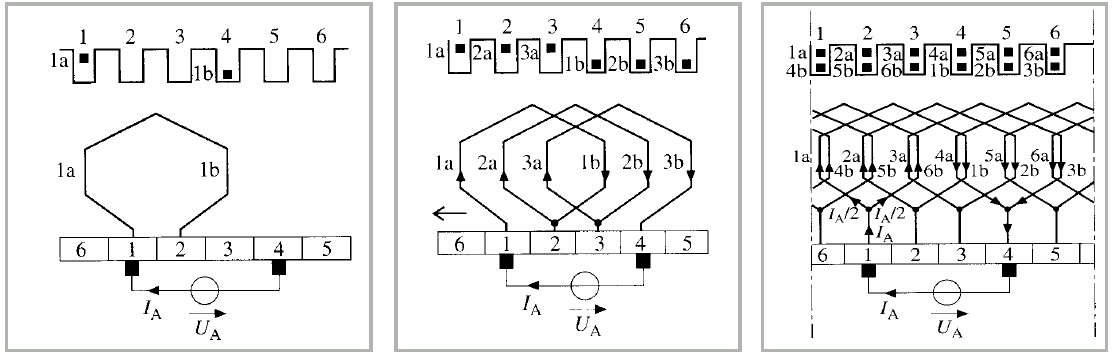
\includegraphics[width=\textwidth]{images/GSM_Wicklungen.png}
	    	\caption{Entstehung einer Schleifenwicklung}
	    \end{subfigure}
	    \begin{subfigure}[t]{0.45\textwidth}
	    	\centering
	    	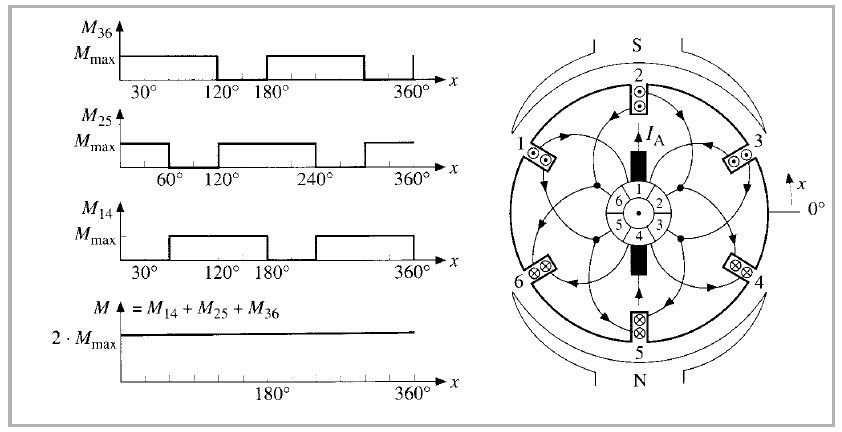
\includegraphics[width=\textwidth]{images/GSM_Drehmomentdarstellung.png}
	    	\caption{Alle Drehmomente zusammen ergeben ein gleichmässiges Drehmoment}
	    \end{subfigure}
    \end{figure}

    
    \subsection{Grundgleichungen}
    \begin{minipage}{15.1cm}
    \begin{tabular}[c]{ | p{6cm} | p{8cm} |}
    	\hline
    	Umfangsgeschwindigkeit & v$_u=\omega\cdot R = 2\pi\cdot n \cdot
    	R=\frac{2\pi\cdot f \cdot R}{p}=2\cdot f \cdot \tau_p = d\cdot\pi\cdot n$\\
    	 & Geometrisch: v$=d\cdot\pi\cdot f$\\
    	\hline
    	Teilspannung eines Leiters & $U_{iL}=2\cdot \tau_p \cdot f \cdot l \cdot
    	B_m= 2\cdot f\cdot \Phi = 2\cdot p \cdot n \cdot \Phi$\\
    	\hline
    	Gesamtspannung & $U_i=\frac{z}{2\cdot a}\cdot U_{iL}=\frac{z}{a}\cdot
    	p \cdot n \cdot \Phi=k_1\cdot\Phi\cdot n = B_m \cdot z \cdot l \cdot v$\\
    	\hline
    	Ankerspannung & $U_a=R_a\cdot I_a + L_a\frac{dI_a}{dt}+U_i = U_i + U_{BK} + I_{AN} \cdot R_A$ \\
    	\hline
    	Erregerspannung & $U_e=R_e\cdot I_e + L_e\frac{dI_e}{dt}$\\
    	\hline
    	Induzierte Spannung & $U_i = k_1\cdot \Phi \cdot \omega_{mech} = B\cdot l
    	\cdot $v$ \quad k_1 = Maschinenkonstante$\\
    	\hline
    	Elektrisch verursachtes Drehmoment & $M_{el}=M_{Welle}+M_{Reibung}+J\cdot\frac{d\omega_{mech}}{dt}=k_1\cdot
    	\Phi\cdot I_a$\\
    	\hline
    	Erregerfluss & $\Phi = \frac{L_e}{N_e}\cdot I_e$\\
    	\hline
    	Ideale Luftspaltleistung & 
    		$P_{Luft}=U_i\cdot I_A = M_{Luft} \cdot \omega $\\
    	\hline
    	Ideales Luftspaltdrehmoment & 
    		$M_{Luft} = N \cdot B \cdot I \cdot d \cdot l$ \\
    	\hline
    	Mech. Leistung an der Welle &
    	$P_{Welle}=P_{Luft}-V_{Fe}-V_{Reib}-V_{zus}$ \quad $V{...} =$ Verluste\\
    	\hline
    	Nenndrehmoment $M_{N}$ & $\frac{P_{Mech}}{2 \cdot \pi n_{0}}$ \qquad Vorsicht $n_0$ nicht in $min^{-1}$!! \\ \hline
    	Ankerwiderstand $R_{A}$ & $R_{A} = \frac{U_{N} - U_{iN}}{I_{N}} $ \qquad $U_{iN} =$ Induzierte Spannung \\ \hline
    \end{tabular}
    \end{minipage}
    \begin{minipage}{5cm}
    \begin{tabular}{|p{4cm}|}
    \hline
	$U_I = U_{Ind} =$ Induzierte Spannung \\
	\hline
	$U_A =$ Ankerspannung\\
	\hline
	$U_E =$ Erregerspannung \\
	\hline
	$k_1 , k_2 =$ Maschinenkonstanten \\
	\hline
	$P_{Luft} = P_{Mech} =$ Mechanische Leistung \\
	\hline
	$n_0$ oder $n_{N0} =$ Leerlaufdrehzahl \\
	\hline
	$n_N =$ Nenndrehzahl \\
	\hline
	
	
	\end{tabular}
	\end{minipage}
    
    	
    
    \subsection{Nebenschlusmaschinen}
    	Nebenschlussmaschinen am starren Netz unterscheiden sich im Betriebsverhalten nicht von fremderregten Maschinen.
    	
    	
        \renewcommand{\arraystretch}{1.5}
        \begin{tabular}[c]{ | p{6cm} | p{11cm} |}
            \hline
            Drehzahl &
            $ n= \frac{U_A}{k_1 \cdot \Phi} - \frac{R_A \cdot M}{k_1 \cdot k_2 \cdot \Phi^2} \sim \frac{U_A}{I_E} - \frac{M}{I_E^2}$ \newline
            $\Longrightarrow $ bei $I_E$ = 0 und $M$ = 0 $n \rightarrow \infty$ \newline 
            $k_1$, $k_2$ sind Maschinenkonstanten \\
            \hline
            Drehmoment &
            $M=\frac{k_2 \cdot \Phi \cdot U_{Anker}}{R_{Anker}} - \frac{k_1 \cdot k_2 \cdot\phi^2 \cdot n}{R_A} =\frac{P_{mech}}{2\pi n_N}=\frac{U_{iN}I_N}{2\pi n_N}\sim I_E \cdot U_A - I_E ^2 \cdot n$
            \quad Achtung: $[n] = s^{-1}$\\
            \hline
            Leistung &
            $P_{Anker}= U_i \cdot I \pm I^2 \cdot R_A $(+ bei Motor; - bei Generator) \\
            \hline
            Anlaufmoment &
            $M_A = \frac{k_1 \cdot \Phi \cdot U}{R_1}$ \\
            \hline
            Magnetischer Fluss des Hauptfeldes & 
            $\Phi=\frac{L_e}{N_e}\cdot\frac{U_a}{R_e+R_v}$\\
            \hline
            Leerlaufdrehzahl &
            $\omega_m=\frac{N_e\left(R_E+R_V\right)}{k_1\cdot
            L_e}-\frac{R_a\left(R_e+R_V\right)^2N_e^2}{\left(k_1L_eU_a\right)^2}\cdot
            M_{el}$\\
            & $n_0 = \frac{U_A}{k_1 \cdot \Phi}$ \\
            & $n_0 = \frac{n_N \cdot U_{Ind,neu}}{U_{Ind,nenn}}$  wenn Verluste $ \approx$ const. !\\
            & $n_0$ ist Näherungsweise nicht Abhängig von $U_A$ \\
            \hline
            
        \end{tabular}
        \renewcommand{\arraystretch}{1.3}
        
    \subsection{Reihenschluss Maschine}
    Auch bekannt als Seriemaschine oder Hauptschlussmaschine\\
        \renewcommand{\arraystretch}{2}
        \begin{tabular}[c]{ | p{6cm} | p{9cm} |}
            \hline
            Drehmoment &
            $ M=  \frac{U_{Induziert} \cdot I_A}{2 \cdot \pi n_N} = \frac{k_1 \cdot k_E \cdot I_A ^2}{2\cdot \pi n_N}= \frac{k_1 \cdot k_E}{2 \cdot \pi n_N}\cdot(\frac{U}{R_A + R_E + k_1 \cdot k_E \cdot n})^2$ \\
            \hline
            Anlaufstrom &
            $I_A=\frac{U_N}{\sum R_a}=\frac{U_N I_N^2}{U_N I-P_N}$ \\
            \hline
            Elektrisch verursachtes Drehmoment & $M_{el}=\frac{L_e}{N_e}k_1\cdot I_a^2$\\
            \hline
            Leerlaufdrehzahl &
            $\omega_m=\frac{N_e}{L_e}\frac{U_a}{k_1I_a}-\frac{N_e}{L_e}\frac{R_a+R_e}{k_1}=\frac{\sqrt{N_e}\cdot
            U_a}{\sqrt{L_ek_1M_{el}}}-\frac{N_e}{L_e}\frac{R_a+R_e}{k_1}$\\
            \hline
            Anlaufdrehmoment bei begrenztem Anlaufstrom & $M^*_A = (\frac{I^*_A}{I_N})^2 \cdot M_N$ \\ \hline
        \end{tabular}
        \renewcommand{\arraystretch}{1.5}
\section{Grundlagen Drehfeldmaschinen}
    \subsection{Dreiphasenwechselstrom (Drehstrom)}
        \begin{minipage}{8cm}
            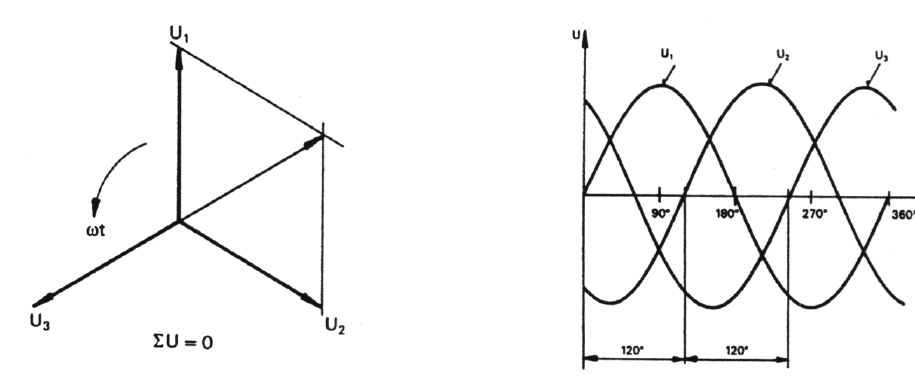
\includegraphics[width=7.5cm]{images/Drehstrom.png}
        \end{minipage}
        \begin{minipage}{10cm}
            Zeiger drehen mit $\omega t$ im Gegenuhrzeigersinn ($\omega > 0$). \\
            $\underline{U}_2$ ist gegenüber $\underline{U}_1$ $120^{\circ}$ nacheilend, $\underline{U}_3$ gegenüber $\underline{U}_1$ $240^{\circ}$.\\
            \\
            Somit gilt (bei symmetrischer Belastung): \\
            $\underline{U}_2 = \underline{U}_1 \cdot e^{j (-120^{\circ})}; \underline{U}_3 = \underline{U}_1 \cdot e^{j (-240^{\circ})} = \underline{U}_1 \cdot e^{j (120^{\circ})}$
        \end{minipage}
    \subsubsection{Stern- (Y) / Dreieckschaltung ($\Delta$)}
        \renewcommand{\arraystretch}{2}
        \begin{tabular}{| p{4.5cm} | l | l |}
            \hline
            &
            Sternschaltung (Y) &
            Dreieckschaltung ($\Delta$) \\
            \hline
            \vspace{0.2cm} &
            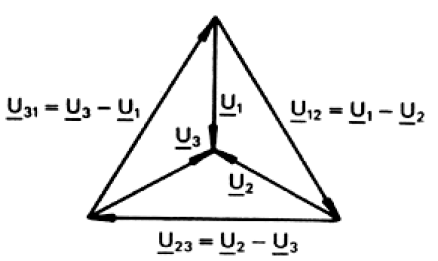
\includegraphics[width=5cm]{images/Sternspannung.png} &
            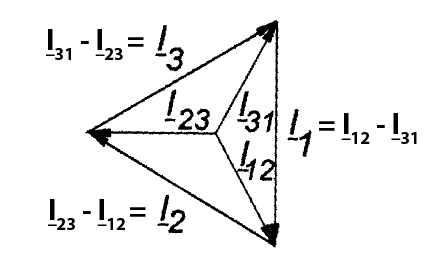
\includegraphics[width=5cm]{images/Dreieckstrom.png} \\
            \hline
            Verkettete Spannung &
            $U = U_{Str} \cdot \sqrt{3}$ \hspace{0.2cm} $\underline{U} = \underline{U}_{Str} \cdot \sqrt{3} \cdot e^{j 30^\circ}$ &
            $U = U_{Str}$ \hspace{0.2cm} $\underline{U} = \underline{U}_{Str}$ \\
            \hline
            Aussenleiterströme &
            $I = I_{Str}$ \hspace{0.2cm} $\underline{I} = \underline{I}_{Str}$ &
            $I = I_{Str} \cdot \sqrt{3} $ \hspace{0.2cm} $\underline{I} = \underline{I}_{Str} \cdot \sqrt{3} \cdot e^{-j 30^\circ} $ \\
            \hline
            Gesamt-Scheinleistung &
            $S = 3 \cdot S_{Str} =\sqrt{3} \cdot U \cdot I $ \hspace{0.2cm} in $[VA]$ &
            $S = 3 \cdot S_{Str} = \sqrt{3} \cdot U \cdot I$ \hspace{0.2cm} in $[VA]$ \\
            \hline
            Scheinleistung pro Strang &
            \multicolumn{2}{l|}{\hspace{3cm} $S_{Str} = U_{Str} \cdot I_{Str}$ \hspace{0.2cm} in $[VA]$} \\
            \hline
            Wirkleistung &
            \multicolumn{2}{l|}{\hspace{3cm} $P = S \cdot \cos\varphi = \sqrt{3} \cdot U \cdot I \cdot \cos\varphi$ \hspace{0.2cm} in $[W]$} \\
            \hline
            Blindleistung &
            \multicolumn{2}{l|}{\hspace{3cm} $Q = S \cdot \sin\varphi = \sqrt{3} \cdot U \cdot I \cdot \sin\varphi$ \hspace{0.2cm} in $[var]$} \\
            \hline
        \end{tabular}
        \renewcommand{\arraystretch}{1.5}

    \subsubsection{Stern-Dreieck-Umwandlung}
        \begin{minipage}[lt]{7.5 cm}
            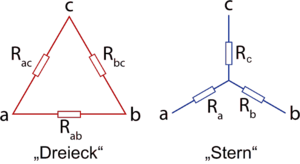
\includegraphics[width=6cm]{images/stern-dreieck.png}
        \end{minipage}
        \begin{minipage}[rt]{9.35 cm} %BASTEL!!
            \renewcommand{\arraystretch}{2}
            \begin{tabular}{ll}
                Umwandlung $\triangle \rightarrow Y$: &
                $Z_{c} = \dfrac{Z_{ac} Z_{bc}}{Z_{ab}+Z_{bc}+Z_{ac}}$ \\
                Umwandlung $Y \rightarrow \triangle$: &
                $Y_{ac}=\dfrac{Y_{a} Y_{c}}{Y_{a}+Y_{b}+Y_{c}}$ \\
                Bei gleichen Widerständen: &
                $R_Y = \frac{R_\triangle}{3}$ \\
                Bei gleichen Kapazitäten: &
                $C_Y = C_\triangle \cdot 3 $ \\
                Bei gleichen Induktivitäten: &
                $L_Y = \frac{L_\triangle}{3}$
            \end{tabular}
            \renewcommand{\arraystretch}{1.5}
        \end{minipage}
        
    \subsection{Feld in einer Drehstrommaschine}
        \begin{minipage}{7cm}
            \abb{images/Drehfeld.png}{6cm}{Entstehung eines Drehfeldes in einem elMaschine}
        \end{minipage}
        \begin{minipage}{11cm}
            Bei einem Drehfeld entsteht zu jedem Zeitpunkt gleichgrosses Magnetisches Feld, woraus dann ein gleichmässiges Drehmoment resultieren kann. Nach dem obrigen Bild dreht sich das Feld in einer Periode um die eigene Achse. Verwendet man mehrere Polpaare wird die Drehzahl reduziert \\
            $Drehfelddrehzahl  = n_d =\frac{f}{p}$ \\
        \end{minipage}

    \subsubsection{Schlupf}
        Als Schlupf bezeichnet man die Beziehung zwischen Drehfelddrehzahl und Läuferdrehzahl. Sie wird mit folgender Formel beschrieben: \\
        \begin{multicols}{2}
            $Schlupf = s = \frac{n_d - n}{n_d}$ \\
            Das heisst bei einer Läuferdrehzahl $<$ $n_d$ in Drehfeldrichtung ist der Schlupf 0 $<$ s $<$ 1
        \columnbreak
        
            \abb{images/Schlupfgerade.png}{4cm}{Schlupfgerade}
        \end{multicols}
        
	\subsubsection{Drehzahl-Drehmoment Kennlinie}
		\begin{center}
			\includegraphics[width=0.4\textwidth]{images/Mn-Kennlinien.png}
		\end{center}        

\section{Drehstrom- Synchronmaschinen(DSM)}
    \subsection{Aufbau der DSM}
        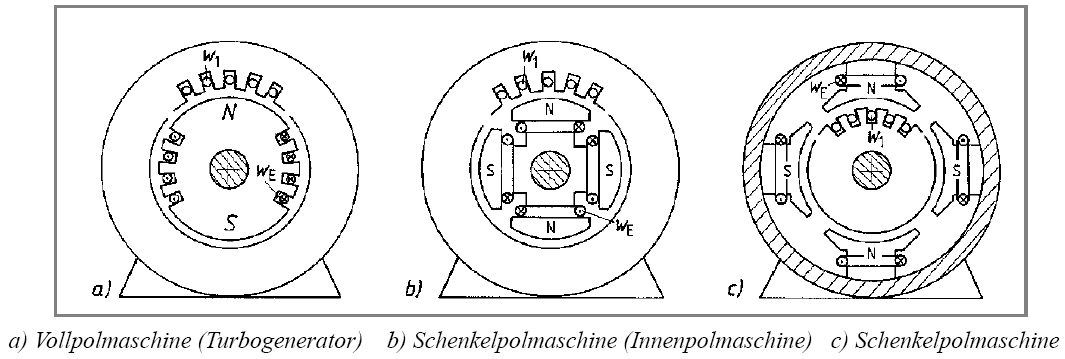
\includegraphics[width=12cm]{./images/Aufbau_DSM.png}\\
        \begin{description}
            \item[Innenpolmaschine:] Der Läufer ist ein Dauermagnet, oder wird mit Gleichstrom und über Schleifer
            zu einem solchem gemacht. Dieser läuft mit dem aussen anliegendem Drehfeld mit.
            \item[Aussenpolmaschine:] Der Läufer erzeugt ein Drehfeld, welches sich immer am konstanten Statorfeld
            ausrichtet. Worauf sich des Läufer dreht.
            \item[Turbomaschine:] Die Schleiferlose Variante. Mit Hilfe eines Hilfsgenerator auf der gleichen Welle
            wird ein Drehstrom erzeugt, welcher auf dem Läufer selbst gleichgerichtet wird. Damit wird dan ein
            konstantes Magnetfeld (Dauermagnet) erzeugt (wie die Innenpolmaschine).
        \end{description}

    \subsection{Ersatzschaltbild}
        \begin{minipage}{11cm}
            \abb{images/Ersatz_DSM.png}{8cm}{Ersatzschaltung DSM}    
            Es gibt 2 Unterteilungen: \\
            \begin{description}
                \item[Wirkleistung:] Gibt die DSM leistung ab oder nimmt sie auf. Zu erkennen ist das am Phasenwinkel
                zwischen $U_{KL}$ und $U_P$. Ist $U_P$ voreilend, so ist es ein \textbf{Generator}, anderseits ein
                \textbf{Motor}.
                \item[Blindleistung:] Blindleistung Auf- oder Abgabe. Bei \textbf{Übererregung} oder auch \textbf{kapazitiven
                Betrieb} gibt der DSM Blindleistung ab. Bei \textbf{Untererregung} oder auch \textbf{induktiven Betrieb}
                nimmt er auf.
            \end{description}
        \end{minipage}
        \begin{minipage}{8cm}
            \abb{images/Zeigerdiagram.png}{6cm}{Betriebszustände einer DSM}
        \end{minipage}\\
      %  \begin{tabular}{lll}
      %  	& Übererregung & Untererregung \\
      %  Motor & & \\
      %  &
      %  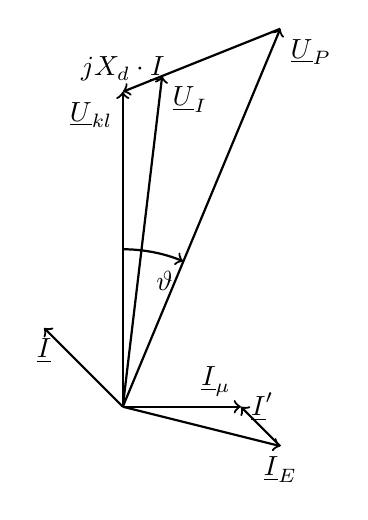
\begin{tikzpicture}[->,thick]
\coordinate (null) at (0,0) {};
\coordinate (I) at (-1,1) {};
\coordinate (Ukl) at (0,4) {};
\coordinate (Up) at (2,4.8) {};
\coordinate (Ie) at (2,-0.5) {};
\coordinate (Iu) at (1.5,0) {};

\draw (null) -- (I) node [anchor=north] {$\underline{I}$};

\draw (null) -- (Ukl) node [anchor=north east] {$\underline{U}_{kl}$};
\draw (null) -- (0.5,4.2) node [anchor=north west] {$\underline{U}_I$};
\draw (null) -- (Up) node [anchor=north west] {$\underline{U}_P$};
\draw (Up) -- (Ukl) node [anchor=south] {$jX_d\cdot\underline{I}$};

\draw (null) -- (Ie) node [anchor=north] {$\underline{I}_E$};
\draw (Ie) -- (Iu) node [anchor=west] {$\underline{I}^\prime$};
\draw (null) -- (Iu) node [anchor=south east] {$\underline{I}_\mu$};

\draw (0,2) arc [radius=2, start angle=90, delta angle=-22.5] node [anchor=north east] {$\vartheta$};
\end{tikzpicture} &
      %  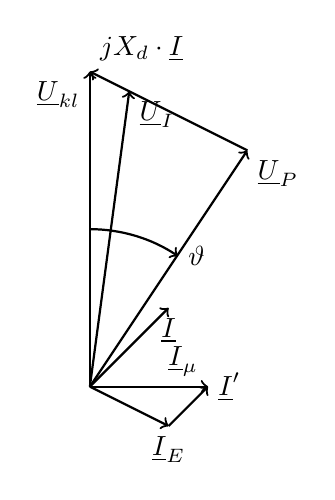
\begin{tikzpicture}[->,thick]
\coordinate (null) at (0,0) {};
\coordinate (I) at (1,1) {};
\coordinate (Ukl) at (0,4) {};
\coordinate (Up) at (2,3) {};
\coordinate (Ie) at (1,-0.5) {};
\coordinate (Iu) at (1.5,0) {};

\draw (null) -- (I) node [anchor=north] {$\underline{I}$};

\draw (null) -- (Ukl) node [anchor=north east] {$\underline{U}_{kl}$};
\draw (null) -- (0.5,3.75) node [anchor=north west] {$\underline{U}_I$};
\draw (null) -- (Up) node [anchor=north west] {$\underline{U}_P$};
\draw (Up) -- (Ukl) node [anchor=south west] {$jX_d\cdot\underline{I}$};

\draw (null) -- (Ie) node [anchor=north] {$\underline{I}_E$};
\draw (Ie) -- (Iu) node [anchor=west] {$\underline{I}^\prime$};
\draw (null) -- (Iu) node [anchor=south east] {$\underline{I}_\mu$};

\draw (0,2) arc [radius=2, start angle=90, delta angle=-34] node [anchor=west] {$\vartheta$};
\end{tikzpicture}\\
      %  Generator & & \\
      %  &
      %  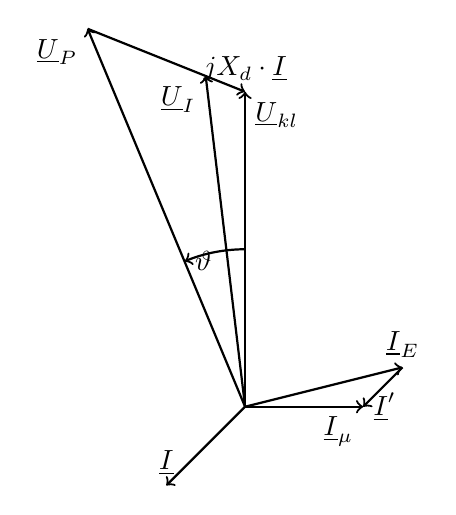
\begin{tikzpicture}[->,thick]
\coordinate (null) at (0,0) {};
\coordinate (I) at (-1,-1) {};
\coordinate (Ukl) at (0,4) {};
\coordinate (Up) at (-2,4.8) {};
\coordinate (Ie) at (2,0.5) {};
\coordinate (Iu) at (1.5,0) {};

\draw (null) -- (I) node [anchor=south] {$\underline{I}$};

\draw (null) -- (Ukl) node [anchor=north west] {$\underline{U}_{kl}$};
\draw (null) -- (-0.5,4.2) node [anchor=north east] {$\underline{U}_I$};
\draw (null) -- (Up) node [anchor=north east] {$\underline{U}_P$};
\draw (Up) -- (Ukl) node [anchor=south] {$jX_d\cdot\underline{I}$};

\draw (null) -- (Ie) node [anchor=south] {$\underline{I}_E$};
\draw (Ie) -- (Iu) node [anchor=west] {$\underline{I}^\prime$};
\draw (null) -- (Iu) node [anchor=north east] {$\underline{I}_\mu$};

\draw (0,2) arc [radius=2, start angle=90, delta angle=22.5] node [anchor=west] {$\vartheta$};
\end{tikzpicture} &
      %  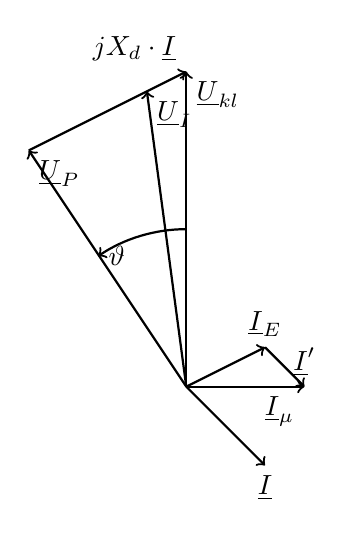
\begin{tikzpicture}[->,thick]
\coordinate (null) at (0,0) {};
\coordinate (I) at (1,-1) {};
\coordinate (Ukl) at (0,4) {};
\coordinate (Up) at (-2,3) {};
\coordinate (Ie) at (1,0.5) {};
\coordinate (Iu) at (1.5,0) {};

\draw (null) -- (I) node [anchor=north] {$\underline{I}$};

\draw (null) -- (Ukl) node [anchor=north west] {$\underline{U}_{kl}$};
\draw (null) -- (-0.5,3.75) node [anchor=north west] {$\underline{U}_I$};
\draw (null) -- (Up) node [anchor=north west] {$\underline{U}_P$};
\draw (Up) -- (Ukl) node [anchor=south east] {$jX_d\cdot\underline{I}$};

\draw (null) -- (Ie) node [anchor=south] {$\underline{I}_E$};
\draw (Ie) -- (Iu) node [anchor=south] {$\underline{I}^\prime$};
\draw (null) -- (Iu) node [anchor=north east] {$\underline{I}_\mu$};

\draw (0,2) arc [radius=2, start angle=90, delta angle=34] node [anchor=west] {$\vartheta$};
\end{tikzpicture}\\
      %  \end{tabular}
      
      \subsubsection{Phasenschieber}
      Ein DSG, der im Idealfall nur Blindleistung mit dem Netz austauscht. In der Praxis müssen die Verluste des DSG(Reibung, Ventilation, Stromwärme etc.) entweder vom Netz oder von einer Antriebsmaschine gedeckt werden.
      Der Phasenschieber kennt folgende Betriebsmodi:
      \begin{itemize}
      \item \textbf{\emph{übererregt}} $(U_p > U_N)$: der DSG gibt Blindleistung ab, verhält sich also bezüglich seiner Klemmen wie ein Kondensator.
      \item \textbf{\emph{untererregt}} $(U_p > U_N)$: der DSG nimmt Blindleistung auf, verhält sich also bezüglich seiner Klemmen wie eine Induktivität.
      \end{itemize}
     
    \subsection{Allgemeine Formeln}
    \begin{tabular}[c]{ | p{6.5cm} | p{11.5cm} |}
    	\hline
    	Polpaarzahl	& $p$\\
    	\hline
    	Drehfeldzahl $[s^{-1}]$ bzw $[min^{-1}]$ & $n_d=\frac{f}{p}$ bzw
    	$n_d=\frac{f\cdot 60}{p}$\\
    	\hline
    	Schlupf $[-]$ & $s=\frac{n_d-n}{n_d}$\\
    	\hline
    	Strang- bzw. Phasenspannung &
    	$\underline{U}_{kl}=\underline{U}_p+\underline{U}_{XD}$\\
    	\hline

    	Spannungsfall über Synchroner Reaktanz & $U_{XD}=jX_d\cdot\underline{I}$
    	\\
    	\hline
    	Leerlauferregerstrom für Nennspannung & $I_{E0N}$\\
    	\hline
    	Lastabhängiger Erregerstrom & $\frac{I_E}{I_{E0N}}=\frac{U_p}{U_{Kl}}$\\
    	\hline
    	Klemmenspannung & $U_{kl} = \frac{U_N}{\sqrt{3}}$\\
    	\hline
    	Polradspannung & $U_p=\sqrt{U_{Kl}^2+X_d^2\cdot I^2+2\cdot U_{Kl}\cdot
    	X_d \cdot I\cdot sin \varphi}$\\
    	\hline
    	Polradspannung im Inselnetz & $U_p=\sqrt{U_{Kl}^2+X_d^2} $\\
    	\hline
    	Elekrischer Lastwinkel oder Polradwinkel gem. ESB & $\vartheta = arg(U_p)$ (Winkel zwischen $U_{p}$ und $U_{kl}$)\\
    	\hline
    	Wirkleistung des DSG & $P_{el}=3\cdot
    	U_{Kl}\cdot\frac{U_p}{X_d}\cdot \sin\vartheta = 3 \cdot U_{Kl} \cdot I \cdot \cos{\varphi}$\\
    	\hline
    	Wirkkomponente des Statorstroms & $I \cdot \cos{\varphi} = \frac{U_p}{X_d} \cdot \sin{\varphi}$ \\
    	\hline
    	Antriebsmoment des DSG & $\begin{aligned}
    								M_{Welle} 	&=\frac{3\cdot60}{2\pi\cdot n \cdot
    								    				\eta}\cdot U_{Kl}\cdot\frac{U_p}{X_d}\cdot\sin\vartheta
    								    		&= \frac{3\cdot60}{2\pi\cdot n \cdot
    								    	    	\eta}\cdot U_{Kl}\cdot I \cdot \cos{\varphi}= \frac{P_{mech}}{\omega} \\
    								    	    &= \frac{\sqrt{3} \cdot U_N \cdot I_N \cdot cos\varphi_N \cdot p}{\eta \cdot 2 \cdot \pi \cdot f_N} 
    								\end{aligned}$\\
    	\hline
    \end{tabular}

    \subsection{Betriebsverhalten}
    	Siehe Abbildung \ref{fig:betriebsverhalten}
    	\begin{figure}[h!]
	    	\centering
	    	\begin{subfigure}[t]{0.45\textwidth}
	    		\centering
	    		\adjustbox{scale=0.8}{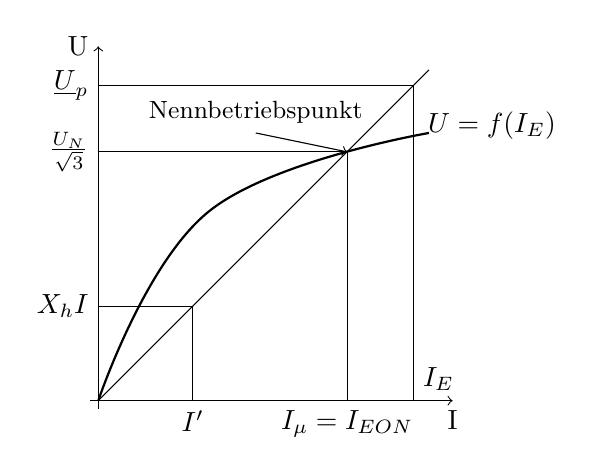
\begin{tikzpicture}
 	\draw[->] (-0.1,0) -- +(4.6,0) node[below] {I};
 	\draw[->] (0,-0.1) -- +(0,4.6) node[left]{U};
 	\draw (0,0) -- +(4.2,4.2);
	\draw[thick]  plot[smooth, tension=.7] coordinates {(0,0) (1.4,2.4) (4.2,3.4)};
	\draw (5,3.5) node[] {$U = f(I_E)$};
	
	\draw (1.2,0) node[below] {$I'$}
		-- ++(0,1.2) 
		-- ++(-1.2,0) node[left] {$X_h I$};
	\draw (3.16,0) node[below] {$I_\mu = I_{EON}$}
		-- ++(0,3.16) 
		-- ++(-3.16,0) node[left] {$\frac{U_N}{\sqrt{3}}$};
	\draw (4,0) node[above right] {$I_E$}
		-- ++(0,4) 
		-- ++(-4,0) node[left] {$\underline{U}_p$};
	\draw[<-] (3.16,3.16) -- (2,3.4) node[above]{\small{Nennbetriebspunkt}};
\end{tikzpicture}}
	    		\caption{Im Betriebspunkt linearisierte Leerlaufgerade}
	    	\end{subfigure}
	    	\begin{subfigure}[t]{0.45\textwidth}
	    		\centering
	    		\adjustbox{scale=0.8}{\begin{tikzpicture}
 	\draw[->] (-0.1,0) -- +(4.6,0) node[below] {$i_E$};
 	\draw[->] (0,-0.1) -- +(0,4.6) node[left]{$\frac{I_k}{I_N}$};
 	\draw (0,0) -- +(4.2,4.2);
	
	\draw (1.8,0) node[below] {$1$}
		-- ++(0,1.8) 
		-- ++(-1.8,0) node[left] {$i_{k0}$};
	\draw (3.6,0) node[below] {$i_{Ek}$}
		-- ++(0,3.6) 
		-- ++(-3.6,0) node[left] {$1$};
\end{tikzpicture}}
	    		\caption{Kurzschlussgerade}
	        \end{subfigure}
	        \caption{Kurven in den Verschiedenen Betriebsarten}
	        \label{fig:betriebsverhalten}
    	\end{figure}
    	
    	\begin{tabular}{ l l p{9cm} }
    		\textbf{Leerlauf}
    		& $I_E = \frac{U_P \cdot \sqrt{3} \cdot I_{E0N}}{U_N}$ 
    		& Die Formel ist für die liniarisierte Gerade \newline
    		  $I_E: $Erregerstrom \newline
    		  $U_P: $verkettete Nennspannung des DS- Netzes\newline
    		  $I_{E0N}:$Leerlauferregerstrom für Nennspannung
    		\\
    		\textbf{Kurzschluss} 
    		& $X_d=\frac{U_P}{I_{K0}}$
    		& Gilt unter Vernachlässigung des Wicklungswiderstand \newline
    		  Die Kurzschlussgerade ist linear
    		\\
    	\end{tabular} 
    	

    \subsubsection{Inselbetrieb}
        \begin{minipage}{10cm}
            \abb{images/Belastungskennlinie_DSM.png}{9cm}{Belastungskennlinie bei konst. Erregerstrom}
        \end{minipage}
        \begin{minipage}{6cm}
            \abb{images/Regulierungslinie_DSM.png}{6cm}{Regulierungskennlinie für konst. $U_{Kl}$}
        \end{minipage} \\
        Die Klemmenspannung nimmt bei kapazitiven Lasten zu, bei induktiven stark ab. Für eine konstante $U_{Kl}$ muss der Erregerstrom wie die Regulierungskennlinie angepasst werden.

    \subsubsection{Netzbetrieb}
        Im Netzbetrieb wird die Frequenz, Klemmenspannung, Umlaufsinn und Phasenlage vom Netz vorgegeben. Das heisst bevor man mit einer DSM ans Netz will, muss man sie so synchronisieren, dass alle jene Parameter mit dem Netz überreinstimmen. Sind die Maschine und Netz synchronisiert und zusammengeschaltet, kann mit Hilfe von $I_E$ und der mechanischen Leistung der Blindstromanteil eingestellt werden: \\
        \begin{minipage}{8.2cm}
            \abb{images/Ortskurve_DSM.png}{8cm}{Ortskurve einer DSM im starren Netz}
        \end{minipage}
        \begin{minipage}{9.7cm}
            \begin{itemize}
                \item Da $U_{Kl} = U_1$ konstant ist, ist der Ursprung des Zeigers $\frac{j \cdot U_p}{X_d}$ immer am gleichen Ort. 
                \item Mit dem Erregerstrom kann man die Länge des Zeigers $\frac{j \cdot U_p}{X_d}$ einstellen.
                \item Die mechanische Leistung ist proportional zum Abstand der Zeigerspitze zur Imaginärachse.
                \item Die Blindleistung ist proportional zum Abstand  der Zeigerspitze zur Reelenachse.
                \item Ist nun die mechanische Leistung konstant und man ändert den Erregerstrom, so wandert die Zeiger auf einer Linie parallel zur Imag-Achse hin und her.
                \item Überschreitet der Zeiger die Stabilitätslinie, schlipft der Läufer durchund es gibt grosse Lärm- und Wärmeentwicklung, da die mechanische Leistung zu gross wird für den Erregerstrom.
                \item Bleibt der Erregerstrom konstant und die mechanische Leistung ändert sich, so wandert der Zeiger auf dem Kreis um (0,$\frac{U_Kl}{j \cdot X_d}$). Jedoch wiederum nur bis zur Stabilitätsgrenze, da dort die Wirkleistung für diesen Erregerstrom maximal ist.
            \end{itemize}
        \end{minipage}
        \\ \\ \\
        $$ U_P = \sqrt{\frac{U^2_{Netz}}{3} + X_d^2 \cdot I^2 + 2 \cdot \frac{U_{Netz}}{\sqrt{3}}\cdot X_d \cdot I \cdot \sin(\varphi)} $$
\section{Drehstrom- Asynchronmaschinen (DAM)}
    \subsection{Aufbau der DAM}
        \begin{tabular}[c]{| p{3cm} | p{5cm} | p{4cm} | p{5cm} |}
            \hline
            Name &
            Aufbau &
            Positiv &
            Negativ \\
            \hline
            Schleifringläufer &
            Ständerwicklung und Läuferwicklung sind für Drehfelder gewickelt. Die Läuferwicklunganschlüsse sind rausgezogen, um einem Widerstand einzuschliessen. &
            Mit deiesem Widerstand lässt sich die Drehzahl regulieren &
            Die Schleifkontakte reduzieren den Wirkungsrad und erhöhen den Verschleiss. \\
            \hline
            Kurzschlussläufer / Käfigläufer &
            Die Läuferwicklungen sind immer kurzgeschlossen. &
            Es kann ein beinahge reibungsloser und verschleisfreier Betrieb ermöglicht werden &
            Die Drehzahl ist beinahe die Drehfeldfrequenz durch die Polzahl \\
            \hline
        \end{tabular}
    \subsection{Funktionsprizip}
        Das vom Ständer erzeugter Drehfeld erzeugt im stillstehenden, kurzgeschlossenen Läufer einen Drehstrom. Der Schlupf ist bei einem stillstehendem Läufer 1. Dieser Drehstrom erzeugt im Läufer ein Drehmoment. Dieses Drehmoment beschleunigt den Läufer.Durch verringert sich Schlupf, was wiederum ein kleineres Drehmoment nachsichtzieht. Bei einem Läufergeschwindigkeit, welche gelcih schnell ist wie das Drehfeld, reslutiert eine relative Geschwindigkeit von 0 (Schlupf von 0)$\rightarrow $ kein Drehmoment. Das heisst der DAM bewegt sich immer mit möglichst kleinem Schlupf.

    \subsection{Ersatzschaltbild}
        Da der DAM nach dem Induktionsgesetz funktionniert, kann man ihn gut als Trafo- Ersatzschaltbild darstellen. Der veränderliche Wirkwiderstand (Lastwiderstand) ist die mechanische Last. Das heisst die Verlustleistung über dem Widerstand ist die Mechanische Nutzleistung (minus die Reibungsverluste). Diese ist, wie man sieht von dem Schlupf abhnängig.
        \abb{images/ersatzschaltbild_DAM}{12cm}{Ersatzschaltbild des DAM mit Last}

     
     
    \subsection{Formeln zur Asynchronmaschine}
    \begin{tabular}[c]{ | p{6cm} | p{9cm} |}
    	\hline
    	Drehfeldzahl $[s^{-1}]$ bzw $[min^{-1}]$ & $n_d=\frac{f}{p}$ bzw
    	$n_d=\frac{f\cdot 60}{p}$\\
    	\hline
    	Schlupf $[-]$ & $s=\frac{n_d-n}{n_d}$\\
    	\hline
    	Zugeführte Wirkleistung & $P_{zu}= P_{el}=3\cdot U_1 \cdot I_1 \cdot
    	\cos\varphi$\\
    	\hline
    	Drehfeldleistung & $P_\delta=P_{el}-3\cdot\left(I_1^2\cdot R_1 +
    	P_{Fe}\right)=3\cdot\frac{R_2^\prime}{s}\cdot I_2^{\prime 2}$\\
    	\hline
    	Wellenleistung ohne Reibung & $P_{mech}=P_\delta-3I_2^{\prime 2}\cdot
    	R_2^\prime=(1-s)\cdot P_\delta$\\
    	\hline
    	Läuferverlustleistung & $P_{v2}=3\cdot R_2^\prime\cdot I_2^{\prime
    	2}=s\cdot P_\delta$\\
    	\hline
    	Drehmoment & $M=\frac{P_{mech}}{2\cdot\pi\cdot
    	n}=\frac{P_\delta}{2\cdot\pi\cdot n_0}$\\
    	\hline
    	Kippmoment & $M_{kipp}=\frac{3\cdot U_I^2}{4\pi\cdot
    	n_1}\cdot\frac{1-\sigma}{R_1(1-\sigma)+\sqrt{R_1^2+X_1^2}}\approx\frac{3\cdot
    	U_1^2}{4\pi\cdot n_1 \cdot X_\sigma}$\\
    	\hline
    	Klosssche Gleichung &
    	$\frac{M}{M_k}=\frac{2}{\left(\frac{s}{s_{kipp}}+\frac{s_{kipp}}{s}\right)}=\frac{2
    	s s_k}{s^2+s_k^2} $\\
    	\hline
    	Kippmoment Dreieckschaltung& $M_k= Faktor \cdot M_N$\\
    	\hline
    	für Sternschaltung & $M_{Stern}= \frac{M_\Delta}{3}$\\
    	\hline
    \end{tabular}
    
    \subsection{Drehmomentkennlinie}
        \begin{minipage}{5cm}
            \abb{images/Drehmomentkenn_DAM.png}{5cm}{$M = f(s)$}   
        \end{minipage}
        \begin{minipage}{13cm}
            $M_K = Kippmoment = Maximales Drehmoment$ \\
            $M_K \approx \frac{3 \cdot U_1^2}{4\cdot \pi \cdot n_1 \cdot X_\sigma}$ \\
            $X_\sigma = X_{\sigma 1} + X_{\sigma 1}^`$ \\
            $\frac{M}{M_K}\approx \frac{2}{\frac{s}{s_k}+\frac{s_k}{s}}$ \\
            $s_k = \frac{R_2^`}{\sqrt{R_1^2 + X_1^2}} \approx \frac{R_2^`}{X_\sigma}$    
        \end{minipage}

        \newpage
    \subsection{Anleitung zur Orskurve des DAM, Heyland-Kreis}
    \begin{enumerate}
      \item Daten für Leerlauf und (echten) Kurzschluss der DAM verifizieren
      bzw. berechnen
      \item Massstäbe festlegen
      \begin{enumerate}
        \item Strommassstab $m_{I_{Ph}}$ Wählen bzw. Tipp befolgen
        \item Leistungsmassstab $m_{P_{gesamt}}=3\cdot U_{Ph}\cdot m_{I_{Ph}}$
        \item Drehmomentsmassstab $m_M=\frac{m_{P_{gesamt}}}{2\pi n_0} =
        \frac{m_{P_{gesamt}}\cdot p}{2\pi f}$
      \end{enumerate}
      \item Konstruktion der Punkte:
      Länge des Strompfeiles in den Zirkel nehmen und Kreis um Ursprung einzeichnen. Zu jedem Punkt die Verluste als Parallele zur $-j$-Achse einzeichnen, Schnittpunkt ergibt den gesuchten Punkt.
      \begin{enumerate}
      	\item Leerlaufpunkt $(s=0)$ aus $P_0$ und $I_0$ bestimmen und in die Grafik $U_{ph},-jI_{Ph}$ eintragen
        \item Anlaufpunkt $(s=1)$ aus $P_{KS}$ und $I_{KS}$ bestimmen und in die Grafik $U_{ph},-jI_{Ph}$ eintragen
      \end{enumerate}
      \item Eisenverlüste $P_{Fe}$ als Parallele zur $-j$-Achse eintragen (z.B. Leistungsaufnahme im Leerlauf)
      \item Mittelsenkrechte der Strecke (Anlaufpunkt-Leerlaufpunkt) bestimmen, Schnittpunkt mit Eisenverlusten $P_{Fe}$: M
      \item Ossanakreis zeichnen
      \item Bremspunkt $s=\infty$ zeichnen: Senkrechte vom Anlaufpunkt auf $-j$-Achse, dann entweder Stromwärmeverluste vom Anlaufpunkt unterteilen in Stator und Rotor oder Anlaufmoment einzeichnen.
      \begin{enumerate}
        \item Anlaufmoment $\rightarrow$ lotrechte Strecke ausgehend vom Anlaufpunkt $(s=1)$ zur $-j$-Achse
        \item Verluste im Rotor und Stator $\rightarrow$ lotrechte Strecke
        ausgehend vom Anlaufpunkt $(s=1)$ zur $-j$-Achse. Tipp: $V=3\cdot I^2\cdot R$
      \end{enumerate}
      \item Schlupfgerade
      \begin{enumerate}
        \item Senkrechte zur Strecke M-Bremspunkt
        \item Skalieren: Schnittpunkt mit der Strecke
        (Bremspunkt-Leerlaufpunkt) ist bei $s=1$
      \end{enumerate}
      Schlupf herauslesen: Verbindung von gegebenem Punkt zum Bremspunkt $s=\infty$, Schnittpunkt mit der Schlupfgerade entspricht dem Schlupf.
      \item $s_N$ einzeichnen je nach Aufgabenstellung
      \begin{enumerate}
        \item Bei Nennstrom gegeben: Kreis mit Stromlänge um Ursprung
        \item Bei Nennleistung gegeben: Senkrechte mit Länge der Leistung
        zwischen Leistungslinie und Ossanakreis
        \item Bei Nennmoment gegeben: Senkrechte mit Länge des Moments zwischen
        Momentenlinie und Ossanakreis
      \end{enumerate}
    \end{enumerate}   

		\begin{sideways}
		
    
\begin{tikzpicture}

	% Bekante Punkte
	\coordinate (pI0) at (1.7,0.4); % I_0
	\coordinate (pPa) at (19:20); % P_A
	\coordinate (pVS) at (0,2);     % Verlust im Stator
	\coordinate (pPosVerlust) at (15,0); % Position an der der Verlust eingetragen wird
	\def\direction{55}; %Winkel von I_N
	
	%Errechnete Punkte
	\coordinate (dirpIn) at ({cos(\direction)},1);
	
	% Koordinatensystem
 	\draw[->] (-1,0) -- ++(23,0) node[below] {$-j$};
  	\draw[->] (0,-1) -- ++(0,17) node[right] {$re$};
  	\path[name path=abszisse] (0,0) -- +(23,0);
  	
  	\clip (-1,-1) rectangle (23,17.5);  % Ganzer Bereich, damit keine Linien weiter gehen.
  	
  	\draw[color=blue, ->] (0,0) -- +(0,10) node[left] {$U_{ph}$};
  
  	% PA und Leistungsline
  	\draw[->] (0,0) -- (pPa) node[above, left=5] {$I_K$};
  	\node at (pPa) [right=0.2cm] {$P_A \quad s=1$};
  	\draw[name path=leistungslinie] (pI0) -- (pPa) node[below, near start, sloped] {Leistungslinie};
  	
  	\draw[color=red, ->] (0,0) -- +(pI0) node[below=0.5cm, midway] {$I_0$};
  	\draw[dashed, name path=eisenverlustlinie] (pI0) -- +(20,0);
  	

  	
  	% Mittelsenkrechte auf der Leistungslinie
  	\begin{scope}
  		\coordinate (pMSLL) at ($ (pI0)!0.5!(pPa) $);
  		\coordinate (pMSLL2) at ($ (pMSLL)!10cm!90:(pI0) $);
  		\path[name path=mittelsenkrechte] (pMSLL) -- (pMSLL2);
  		\path [name intersections={of= mittelsenkrechte and eisenverlustlinie}] (intersection-1) coordinate (pM);
  		\draw[dashed, shorten >=-10pt] (pMSLL) -- (pM);
  		\node[draw, blue, name path global=kreis] at (pM) [circle through=(pI0)] {};
  		\path (pM) node[below] {$M$};
  		\draw ($(pMSLL)!3mm!(pMSLL2)$) to[bend right=45] ($(pMSLL)!3mm!(pPa)$);
  		\path ($(pMSLL)!1.4mm!(pMSLL2)!1.4mm!(pPa)$) node {.};
	\end{scope}
	
	% P_infty berechnen und zeichenen
	\begin{scope}
		\coordinate (pSchnitt) at ($ (pI0) + (pVS) + (pPosVerlust) $);
		\path[name path global= momentlinie] (pI0) -- ($(pI0)!2!(pSchnitt)$);
		\path[name intersections={of= kreis and momentlinie, name=s}] (s-1) coordinate (pPinf);
		\draw[->] (pI0) -- (pPinf) node[near start, below, sloped] {Momentenlinie};
		\draw[dashed] (pM) -- (pPinf);
		\path (pPinf) node[right=0.2cm] {$P_\infty \quad s=\infty$};		
	\end{scope}
	
	% Senkrechte auf MP_infty
	\begin{scope}
		\coordinate (pMMP) at ($ (pM)!0.67!(pPinf) $);
  		\coordinate (pMMP2) at ($ (pMMP)!16cm!90:(pPinf) $);
  		\draw[shorten < = -10cm, ->, name path=skala] (pMMP) -- (pMMP2);
  		\path[name intersections={of= skala and momentlinie, name=sk0}] (sk0-1) coordinate (pSkala0);
  		\draw ($(pMMP)!-3mm!(pMMP2)$) to[bend right=45] ($(pMMP)!3mm!(pPinf)$);
  		\path ($(pMMP)!-1.4mm!(pMMP2)!1.4mm!(pPinf)$) node {.};
	\end{scope}
	
	% Verlängerung von P_inf-Pa
	\begin{scope}		
		\draw[dashed, name path=PinfPa] (pPinf) -- ($(pPinf)!5!(pPa)$);
		\path[name intersections={of=PinfPa and skala, name=sk1}] (sk1-1) coordinate (pSkala1);	
	\end{scope}
	
	% Skala
	\begin{scope}
		\foreach \x in {0.0,0.1,0.2,0.3,0.4,0.5,0.6,0.7,0.8,0.9,1.0} {
			\draw ($(pSkala0)!\x!(pSkala1)$) node[left=2] {\x};
			\draw ($(pSkala0)!\x!(pSkala1)- (-.1,0)$) -- ($(pSkala0)!\x!(pSkala1)- (.1,0)$);
		}
	\end{scope}
	
	% M - S_k
	\begin{scope}
		\coordinate (pSSK) at ($(pI0)!(pM)!(pPinf)$);
		\path[name path=skline] (pM) -- ($(pM)!17cm!(pSSK)$);
		\path[name intersections={of= kreis and skline, name=intersSk}] (intersSk-1) coordinate (pSk);
		\draw[dashed] (pM) -- (pSk) node[above] {$S_K$};
		\draw ($(pSSK)!3mm!(pM)$) to[bend right=45] ($(pSSK)!3mm!(pPinf)$);
  		\path ($(pSSK)!1.4mm!(pM)!1.4mm!(pPinf)$) node {.};
	\end{scope}
	
	% Beschriftung P_zu0
	\coordinate (pPzu00) at ($ (pI0)+ (4,0) $);
	\coordinate (pPzu01) at ($ (0,0)!(pPzu00)!(15,0) $);
	\draw[<->] (pPzu00) -- (pPzu01) node[midway, right] {$P_{zu_0}$};
	
	% Beschriftung M_K
	\path[name path=mkbeschriftung] (pSk) -- +(0,-20);
	\draw[name intersections={of= mkbeschriftung and momentlinie, name=intersMk}, <->] (pSk) -- (intersMk-1) node[midway, left] {$M_K$};

	% I_N
	\begin{scope}
		\coordinate (pINN) at (dirpIn);%($(pI0)!(pM)!(pPinf)$);
		\path[name path=inline] (0,0) -- ($(0,0)!17cm!(pINN)$);
		\path[name intersections={of= kreis and inline, name=intersIn}] (intersIn-1) coordinate (pIN);
		\draw (0,0) -- (pIN) node[left] {$I_N$};
	\end{scope}
	\draw [->] (0,3) arc (90:{\direction+5}:3) node[below left] {$\varphi$};
	% Beschriftung Pmech
	\path[name path=pmech] (pIN) -- +(0,-20);
	\path[name intersections={of= pmech and leistungslinie, name=intersPmech}] (intersPmech-1) coordinate (pPmech);
	\draw [<->] (pIN) -- (pPmech) node[midway, right] {$P_{mech}$};
	%Beschriftung PV
	\path[name path=pv] (pPmech) -- +(0,-20);
	\path[name intersections={of= pv and abszisse, name=intersPv}] (intersPv-1) coordinate (pPv);
	\draw [<->] (pPmech) -- (pPv) node[above right] {$P_V$};
	
  	%Senkrechte von PA herunter
  	\path[name path=pVRotor] (pPa) -- +(0,-20);
	\path[name intersections={of= pVRotor and momentlinie, name=intersPVRotor}] (intersPVRotor-1) coordinate (pPVRotor);
	\draw [<->] (pPa) -- (pPVRotor) node[midway, right] {Stromwärmeverlust Rotor};
  	%Senkrechte von PA herunter Teil 2
  	\path[name path=pVStator] (pPVRotor) -- +(0,-20);
	\path[name intersections={of= pVStator and eisenverlustlinie, name=intersPVStator}] (intersPVStator-1) coordinate (pPVStator);
	\draw [<->] (pPVRotor) -- (pPVStator) node[midway, right] {Stromwärmeverlust Stator};
	 %Senkrechte von PA herunter Teil 3
  	\path[name path=pVEisen] (pPVStator) -- +(0,-20);
	\path[name intersections={of= pVEisen and abszisse, name=intersPVEisen}] (intersPVEisen-1) coordinate (pPVEisen);
	\draw [<->] (pPVStator) -- (pPVEisen) node[midway, right] {Eisenverluste};
	
	
\end{tikzpicture}
		\end{sideways}
	
	
	        \newpage

%   \texttt{ \subsection{Ortskurve des DAM, Heyland- Kreis}
%        \begin{minipage}{9cm}
%            \abb{images/Heylandkreis.png}{8cm}{Heylandkreis mit Leistungs- und Momenteneinteilung}
%        \end{minipage}
%        \begin{minipage}{8cm}
%            \abb{images/Heylandkreis_schlupf.png}{7cm}{Heylandkreis mit Schlupfskalierung}
%        \end{minipage} \\
%        \begin{minipage}{10.5cm}
%            \begin{enumerate}     
%                \item Den Massstab für den Strom wählen zB. $m_I=\frac{0.2 A}{mm}$
%                \item Den Massstab für die Leistung berechnen: $P_{gesamt}=3U_N I_{Ph}$ $m_P=3U_N m_I$
%                \item Den Massstab für das Drehmoment berechnen: $M=\frac{P_\delta}{2\pi n_0};$  $m_M= \frac{p\cdot m_P}{2\pi f}$  p = Polpaar
%                \item $s=0 \rightarrow s_{0}$ messen und einzeichnen
%                \item $s=1 \rightarrow s_{1}$ messen und einzeichnen
%                \item Verlustleistung bei $s_{0}$ herauslesen ($P_{Fe}$) (ev. wenn nicht schon getan, mit \\ $P_{FE} = U \cdot I_{Wirk}$ den Leistungs-Massstab bestimmen.)\\
%                \item $\perp$ vom Mittelpunkt von $\overline{s_{0}s_{1}}$
%                \item Schnittpunkt auf $s_{0}- Achse (Richtung -j) = M$
%                \item Kreis um M mit Schnittpunkt $s_{0}$ und $s_{1}$
%                \item $I_N =$ Tangente auf dem Kreis vom Ursprung (0,0)
%                \item $P_{v1}$ bei $s_{1}$ ausrechnen = $P_{R_1}$ von der Parallele zur J-Achse, welche durch M geht nach oben abtragen.
%                \item Verbindung des Punktes zu $s_{0}$ verlängern $\rightarrow$ $s_{\infty}$
%                \item \textit{ Bei Vereinfachung $R_{Cu}=0:\\ s_{0}$ auf Imaginär- Achse; $s_{\infty}$ auf Imaginär-Achse}
%                \item Schlupf- Skalierung: $\perp$ auf $\overline{s_{\infty}M}$
%                \item Schnittpunkt mit Verlängerung $\overline{s_{1}s_{\infty}}= 1$
%                \item Schnittpunkt mit $\overline{s_{0}s_{\infty}}= 0$
%                \item Dazwischen lineare Unterteilung
%            \end{enumerate}
%        \end{minipage}
%        \begin{minipage}{7cm}
%            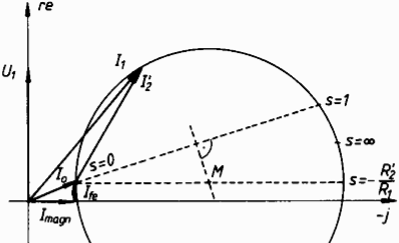
\includegraphics[width=6cm]{../ElMasch/images/StromortskurveDAM.png}\\
%            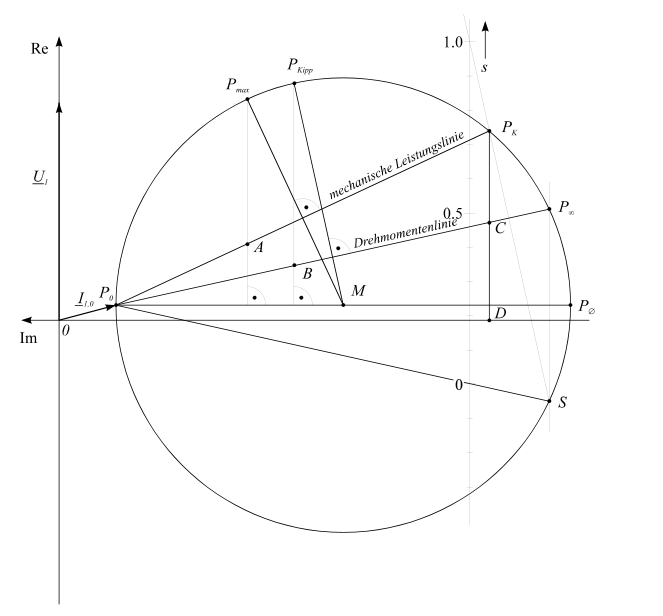
\includegraphics[width=8cm]{../ElMasch/images/OssannakreisPkipp.png}
%        \end{minipage}}
\section{Antriebstechnik}

\subsection{Gradlinige Bewegungen}
\begin{tabular}[c]{ | p{5cm} | p{8cm} | p{4cm} | }
	\hline
	Kraft & $F=m\cdot a=m\cdot\frac{dv}{dt}$ & N \\
	\hline
	Leistung & $P=v\cdot F$ & W \\
	\hline
	Kinetische Energie & $W_{kin}=\frac{1}{2}\cdot m \cdot v^2$ & Ws \\
	\hline
\end{tabular}

\subsection{Rotierende Bewegungen}
\begin{tabular}[c]{ | p{5cm} | p{8cm} | p{4cm} | }
	\hline
	Winkelgeschwindigkeit & $\omega = 2\cdot\pi\cdot n$ & $s^{-1}$ \\
	\hline
	Geschwindigkeit & $v=\omega \cdot r = 2 \cdot\pi\cdot n \cdot r$ &
	$\frac{m}{s}$
	\\
	\hline
	Leistung & $P=\frac{M}{r}\cdot 2 \cdot\pi\cdot n \cdot r = 2\cdot\pi\cdot n
	\cdot M = \omega \cdot M$ & W \\
	\hline
	Kinetische Energie & $W_{kin}=\frac{1}{2}\cdot J \cdot\omega^2$ & Ws \\
	\hline
\end{tabular}

\subsection{Massenträgheit und Beschleunigung}
\begin{tabular}[c]{ | p{5cm} | p{8cm} | p{4cm} | }
	\hline
	Trägheitsmoment & $J=\int\limits_{0}^mr^2\cdot dm$ & $kgm^2$ \\
	\hline
	Beschleunigungsmoment & $M_B=J\cdot\alpha = J\cdot\frac{d\omega}{dt}=J\cdot
	2\pi\cdot\frac{dn}{dt}$ & Nm\\
	\hline
	Energieaufwand für die Beschleunigung & $W=\frac{1}{2}\cdot J \cdot
	\left(\omega_2^2-\omega_1^2\right) = \frac{1}{2}\cdot
	m\cdot\left(v_2^2-v_1^2\right)$ & Ws\\
	\hline
\end{tabular}

\subsection{Umrechnen der Bewegungsgrössen auf die Motorwelle}
\begin{tabular}[c]{ | p{14cm} | p{3.5cm} | }
	\hline
	Übersetzungsverhältnis des Getriebes & $i=\frac{n_1}{n_2}$\\
	\hline
	Moment der Lastmaschine, auf die Motorwelle umgerechnet &
	$M_1=\frac{M_2}{\eta_G}\cdot\frac{n_2}{n_1}$\\
	\hline
	Trägheitsmoment der Lastmaschine, auf die Motorwelle umgerechnet &
	$J_1=\frac{J_2}{\eta_G\cdot i^2}$\\
	\hline
	Ersatzmoment einer Masse m, die sich gradlinig mit v bewegt, bezogen auf eine
	Welle mit $\omega$ & $M_{ers}=\frac{F\cdot v}{\omega}=F\cdot r_{ers}$\\
	\hline
	Ersatzträgheitsmoment einer Masse m & $J_{ers}=m\cdot r_{ers}^2$ \\
	\hline
\end{tabular}

\subsection{Beschleunigungsvorgänge}
\begin{tabular}[c]{ | p{9cm} | p{8.5cm} | }
	\hline
	Dynamisches Grundgesetz der Antriebstechnik & $J\cdot\frac{d\omega}{dt}= \sum
	M(\omega)=M_{Mot(\omega)}+M_{Last(\omega)}$\\
	\hline
	Stationärer Lastfall & $\sum M=0=M_{Mot}+M_{Last}$\\
	\hline
	Zeitbedarf für eine Drehzahlerhöhung von $\omega_1$ auf $\omega_2$ &
	$t_{an}=J\int\limits_{\omega_1}^{\omega_2}\frac{1}{M_B}\cdot d\omega$ \\
	\hline
	Bei konstantem Beschleunigungsmoment &
	$t_{an}=\frac{J}{M_b}\cdot\left(\omega_2-\omega_1\right)$ \\
	\hline
	Winkelgeschwindigkeit entsprechend Nenndrehzahl $n_N$ & $\omega_N$\\
	\hline
	Bei linear abnehmendem Beschleunigungsmoment &
	$t_{an}=\frac{J}{M_{B_{max}}}\cdot\omega_N\cdot\int\limits_{\omega_1}^{\omega_2}\frac{1}{\omega_N-\omega}\cdot
	d\omega$ \\
	\hline
	Für $\omega_1 < \omega_2 < \omega_N$ &
	$t_{12}=\frac{J}{M_{B_{max}}}\cdot\omega_N\cdot
	ln\frac{\omega_N-\omega_1}{\omega_N-\omega_2}$ \\
	\hline
	Anlaufkonstante & $T_an$\\
	\hline
	Stillstand zur Nenndrehzahl $\omega_N$ & $t{an}\approx 5\cdot T_{an}\approx
	5\cdot\omega_N\cdot\frac{J}{M_{B_{max}}}$\\
	\hline
\end{tabular}

\subsection{Stabilität von Arbeitspunkten}
Der stationäre Betriebspunkt eines Antriebs ist durch den Schnittpunkt der
M-n-Kennlinien von Motor und Antriebsmaschine gekennzeichnet\\
\begin{tabular}{ll}
$M=-M_W$\\
$M$ & Motormoment\\
$M_W$ & Lastmoment\\
\end{tabular}\\
Ein Arbeitspunkt ist stabil, wenn bei einer virtuellen Drehzahlerhöhung das
Widerstandsmoment $M_W$ grösser ist als das Motormoment $M$, d.h. einer
Drehzahlerhöhung entgegenwirkt\\
$$\frac{\Delta M- \Delta M_W}{\Delta \omega}<0$$\\

\end{document}
